\documentclass[a4paper,12pt]{article}
\usepackage[T1]{fontenc}
\usepackage[utf8]{inputenc}
\usepackage[spanish]{babel}
\usepackage{graphicx}
\usepackage{fancyhdr}
\usepackage{float}
\usepackage{tipa}
\usepackage{gensymb}
\usepackage{ amssymb }

\topmargin -1.5cm
\textheight 25cm
\oddsidemargin -0.5cm
\textwidth 170mm


\begin{document}

\begin{titlepage}
\pagestyle{fancy}

\begin{center}
\begin{figure}[H]
\begin{center}

\includegraphics[width=250pt]{imagenes/logoUTN.png}
\end{center}
\end{figure}

\vspace*{0.3in}

\begin{LARGE}
\textbf{UNIVERSIDAD TECNOLOGICA NACIONAL}
\end{LARGE}

\vspace*{0.30in}

\begin{Large}
\textbf{FACULTAD REGIONAL BUENOS AIRES}
\end{Large}

\vspace*{0.15in}

\begin{large}
DEPARTAMENTO DE INGENIERIA ELECTRONICA
\end{large}

\vspace*{1in}

\begin{LARGE}
\underline{\textbf{ANÁLISIS DE SEÑALES Y SISTEMAS}}
\end{LARGE}
%\rule{80mm}{0.1mm}

\vspace*{1in}

\begin{Large}
\textbf{Ejercicios de modelización}\\
\end{Large}
2019
\end{center}

\end{titlepage}

%Header and foot
%\normalsize
\pagestyle{fancy}
\lhead{Análisis de Señales y Sistemas \\ Curso R2072}
\chead{
\includegraphics[width=7mm]{imagenes/Logo.jpg}}
\rhead{Universidad Tecnológica Nacional\\ Facultad Regional Buenos Aires}
\lfoot{Modelización de sistemas físicos}
\rfoot{Francisco J. Bernárdez}
\renewcommand{\footrulewidth}{0.4pt} % grosor de la línea del pie

%Add separation
%\null

%\begin{center}
%\huge{\textsc{Modelización de Sistemas Físicos}}\\
%\LARGE{\textsc{"text"}}\\
%\end{center}

%\vspace*{0.3in}

%\begin{figure}[H]
%\begin{center}
%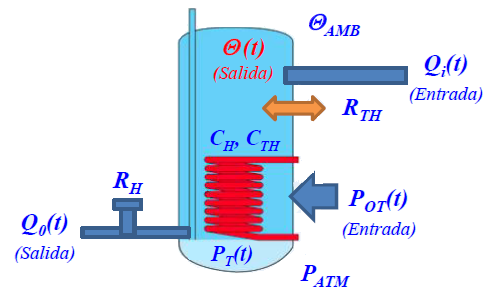
\includegraphics[width = 300pt]{imagenes/termo.png}
%\caption{\small Termotanque. }
%\label{red}

%\end{center}
%\end{figure}

%\vspace*{0.7in}

%\begin{figure}[H]
%\begin{center}
%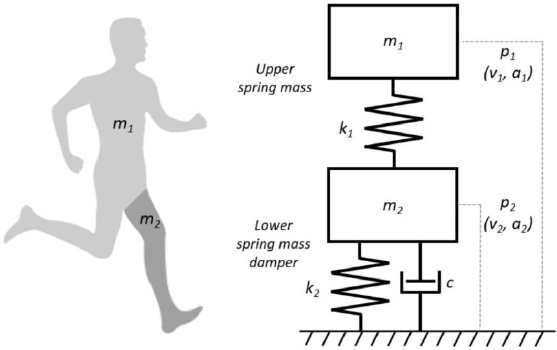
\includegraphics[width = 300pt]{imagenes/cuerpoHumano.png}
%\caption{\small Soporte de la pierna del cuerpo humano.}
%\label{red}
%\end{center}
%\end{figure}

\newpage





%%%%%%%%%%%%%%%%%%%%%
\section{Termotanque}

Este modelo consta de dos sistemas a analizar por separado:
\begin{itemize}
\item Hidraulico: valor para el que se estabiliza el flujo de salida $Q_{o}(t)$ gracias al flujo de entrada $Q_{i}(t)$. 
\item  Termico: valor de la temperatura alcanzada por el tanque gracias a la potencia de entrada $P_{ot}(t)$.
\end{itemize}
Donde las señales de entradas son:\par
\begin{center}

\begin{equation}
Q_{i}(t)=2u(t)
\end{equation}\par
\begin{equation}
P_{ot}(t)=6[\rho(t)-\rho(t-1)]
\end{equation}
\end{center}

y los datos:\par

%datos
\begin{center}
\begin{tabular}{|c | c | c |}
  
  \hline magnitud & valor & unidades \\
  \hline \Theta_{AMB} & 20 & \celsius \\
  \hline P_{ATM} & 0 & $N/m^2$ \\
  \hline C_{TH} & 2 & $Ws$/\celsius \\
  \hline R_{TH} & 0.5 & \celsius/$W$ \\
  \hline C_{H} & 5 & $m^5/N$ \\
  \hline R_{H} & 0.8 & $Ns/m^5$ \\
  \hline 
  
\end{tabular}
\end{center}

\vspace*{0.3in}
\textbf{Nota:} para el analisis y modelado de los sistemas se emplean analogias electricas de los mismo, aunque esto no es una condicion necesaria. Ademas, para la resolucion de las ecuaciones diferenciales se utiliza el metodo: $S_{General}=S_{Homogena}+S_{Particular}$ \par

\begin{figure}[H]
\begin{center}
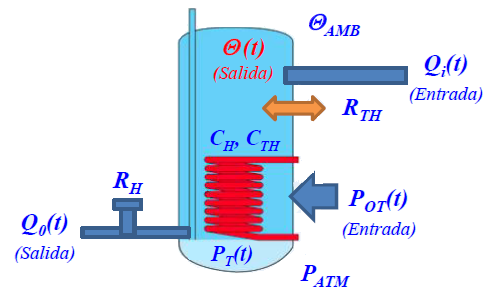
\includegraphics[width = 300pt]{imagenes/termo.png}
\caption{\small Termotanque. }
\label{red}

\end{center}
\end{figure}
\newpage

\subsection{Hidraulico}

Para realizar la equivalencia electrica se tiene en cuenta que el flujo total de agua entregada al modelo es en primera instancia contenido por el termotanque (capacitor) mientras drena a través de una llave de paso (resistencia).\par
Por lo tanto la $corriente$ se corresponde con el flujo de agua recibido, mientras que el $potencial$ con la presión hidraulica P_{h}.\par
\vspace*{0.2in}
El circuito resultante sera:\par

\begin{figure}[H]
\begin{center}
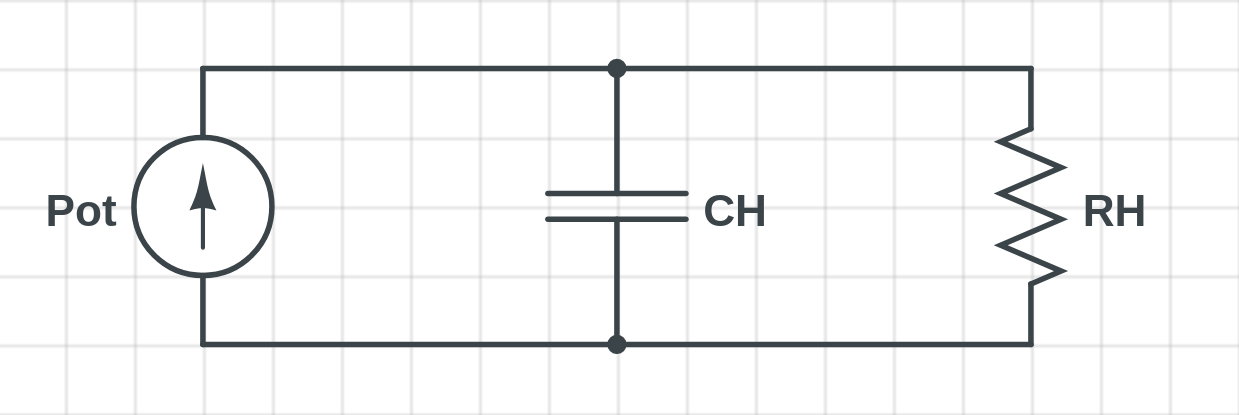
\includegraphics[width = 300pt]{imagenes/RC_hidraulico.png}
\caption{\small Analogia electrica del sistema hidraulico. }
%\label{red}
\end{center}
\end{figure}

Aplicando la primera ley de Kirchhoff y con las consideraciones mensionadas la ecuacion diferencial del modelo resulta:\par

\begin{equation}
Q_{i}(t)= C_{H}\frac{d}{dt}P_{h}+\frac{1}{R_{H}}P_{h}
\end{equation}\par

Normalizando al termino de mayor orden resulta:\par

\begin{equation}
\frac{Q_{i}(t)}{C_{H}}=\frac{d}{dt}
P_{h}+\frac{1}{R_{H}.C_{H}}P_{h}
\end{equation}

\vspace*{0.2in}
La señal de entrada se corresponde con una función constante, lo que simplifica el analisis.\par
\vspace*{0.2in}

\textbf{Solucion particular}\par
\vspace*{0.1in}
La solucion propuesta sera:\par


\begin{equation}
S_{particular}=A
\end{equation}

y su derivada:

\begin{equation}
\frac{d}{dt}S_{particular}=0
\end{equation}

por lo tanto:\par

\begin{equation}
\frac{Q_{i}(t)}{C_{H}}=0+A
\end{equation}

reemplazando:\par

\begin{equation}
S_{particular}=\frac{8}{5}
\end{equation}

\newpage

\textbf{Solucion homogenea}\par
\vspace*{0.2in}
Para la solucion homogenea se propone:\par

\begin{equation}
S_{Homogenea}=Ae^{\leftthreetimes t}
\end{equation}

y su derivada:

\begin{equation}
\frac{d}{dt}S_{Homogenea}=\leftthreetimes A e^{\leftthreetimes}
\end{equation}

su polinomio caracteristico sera:

\begin{equation}
A e^{\leftthreetimes}(\leftthreetimes + \frac{1}{4})=0
\end{equation}

por lo tanto:\par

\begin{equation}
S_{Homogenea}=A e^{-\frac{1}{4}t}
\end{equation}

\vspace*{0.2in}

\textbf{Solucion General}\par
\vspace*{0.2in}

La solucion general resultante sera:\par

\begin{equation}
S_{General}=A e^{-\frac{1}{4}t} + \frac{8}{5}
\end{equation}

\vspace*{0.2in}
El valor de la constante $A$ depende de las condiciones de borde. Considerando $t=0$ entonces:

\begin{equation}
S_{General}(t=0)= A + \frac{8}{5}
\end{equation}

\begin{equation}
A=-\frac{8}{5}
\end{equation}

por lo tanto:\par

\begin{equation}
S_{General}=-\frac{8}{5}e^{-\frac{1}{4}t} +\frac{8}{5}
\end{equation}

\subsection{Grafico}

\vspace*{0.3in}

\begin{figure}[H]
\begin{center}
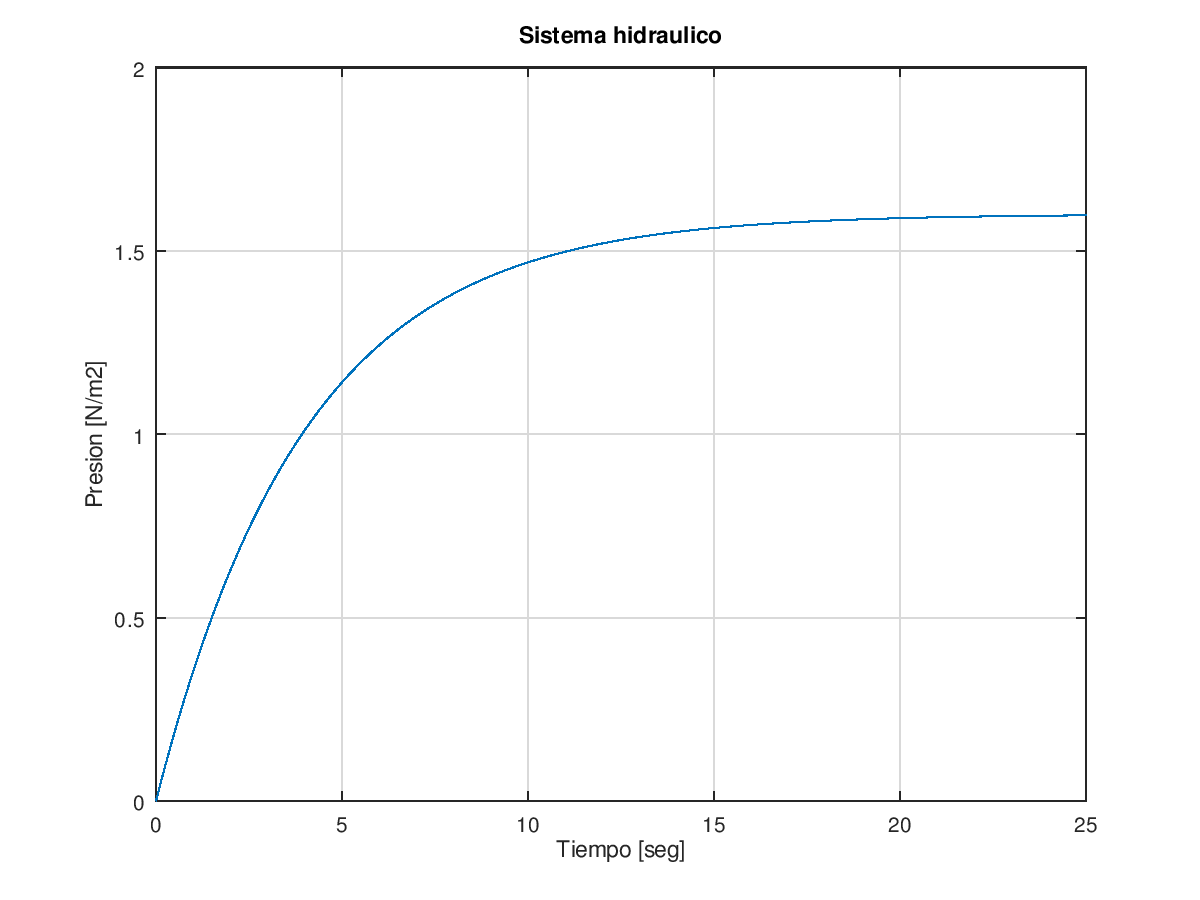
\includegraphics[width = 400pt]{imagenes/termotanqueHidraulico.png}
\caption{\small Comportamiento del sistema Hidraulico.}
\label{red}
\end{center}
\end{figure}











\newpage

\subsection{Termico}
Para realizar la equivalencia electrica se tiene en cuenta que el sistema intentará almacenar la potencia entregada al mismo en el termotanque (capacitor), aunque inevitablemente parte de esta energia se disipa en el medio sin posibilidad de recuperarla (resistencia).\par
Por lo tanto la $corriente$ se corresponde con la potencia de entrada, mientras que el $potencial$ con la temperatura.\par

\vspace*{0.2in}

\textbf{Nota:} Los calculos y graficos del modelo se considerar respecto a la tempratura ambiente.\par

\vspace*{0.3in}
El circuito resultante sera:\par

\begin{figure}[H]
\begin{center}
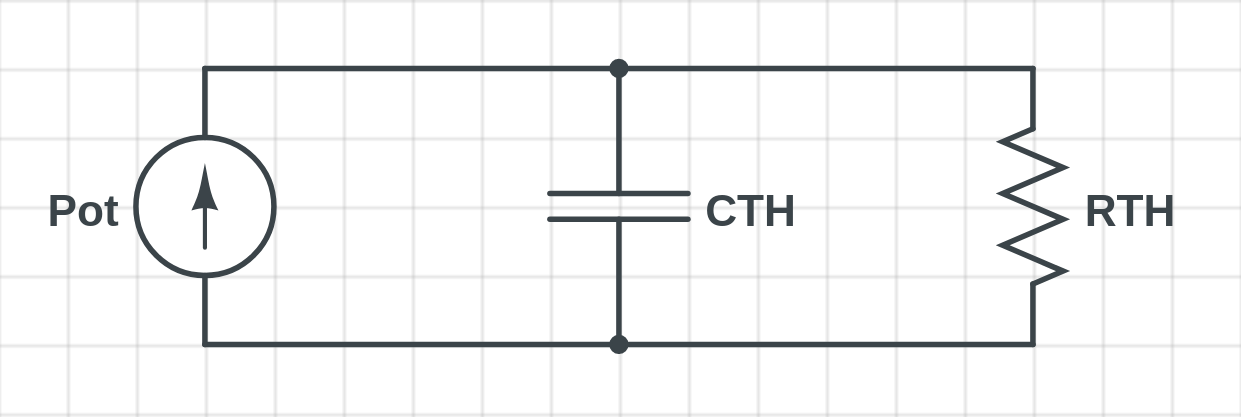
\includegraphics[width = 300pt]{imagenes/RC_termico.png}
\caption{\small Analogia electrica del sistema termico. }
%\label{red}
\end{center}
\end{figure}

Aplicando la primera ley de Kirchhoff y con las consideraciones mensionadas la ecuacion diferencial del modelo resulta:\par

\begin{equation}
P_{ot}(t)= C_{TH}\frac{d}{dt}\Theta+\frac{1}{R_{TH}}\Theta
\end{equation}\par

Normalizando al termino de mayor orden resulta:\par

\begin{equation}
\frac{P_{ot}(t)}{C_{TH}}=\frac{d}{dt}
\Theta+\frac{1}{R_{TH}.C_{TH}}\Theta
\end{equation}

\vspace*{0.2in}

Debido a la señal de entrada $P_{ot}(t)=6[\rho(t)-\rho(t-1)]$ para la resolución se opta por fraccionar el dominio del tiempo en dos intervalos:
\begin{itemize}
\item $0 \leq t_{1} \leq 1$
\item $1 \leq t_{2} \leq \infty$
\end{itemize}

\subsubsection{Intervalo $0 \leq t_{1} \leq 1$}
\vspace*{0.3in}
\textbf{Solucion particular}\par
\vspace*{0.3in}
Para este intervalo la señal de entrada $P_{ot}(t)$ se corresponde con una funcion lineal, por lo que la solucion propuesta sera:\par

\begin{equation}
S_{particular}=At+B
\end{equation}

y su derivada:

\begin{equation}
\frac{d}{dt}S_{particular}=A
\end{equation}

por lo tanto:\par

\begin{equation}
\frac{P_{ot}(t)}{C_{TH}}=A+(At+B)
\end{equation}

reemplazando:\par

\begin{equation}
S_{particular}=3t-3
\end{equation}

\vspace*{0.1in}

\textbf{Solucion homogenea}\par
\vspace*{0.2in}
Para la solucion homogenea se propone:\par

\begin{equation}
S_{Homogenea}=Ae^{\leftthreetimes t}
\end{equation}

y su derivada:

\begin{equation}
\frac{d}{dt}S_{Homogenea}=\leftthreetimes A e^{\leftthreetimes}
\end{equation}

su polinomio caracteristico sera:

\begin{equation}
A e^{\leftthreetimes}(\leftthreetimes + 1)=0
\end{equation}

por lo tanto:\par

\begin{equation}
S_{Homogenea}=A e^{-t}
\end{equation}

\vspace*{0.2in}

\textbf{Solucion General}\par
\vspace*{0.2in}

La solucion general resultante sera:\par

\begin{equation}
S_{General}=A e^{-t} + 3t-3
\end{equation}

El valor de la constante $A$ depende de las condiciones de borde. Considerando $t=0$ entonces:

\begin{equation}
A=3
\end{equation}

por lo tanto:\par

\begin{equation}
S_{General}=3 e^{-t} + 3t-3
\end{equation}


\subsubsection{$1 \leq t_{2} \leq \infty$}
\vspace*{0.3in}
\textbf{Solucion particular}\par
\vspace*{0.1in}

Para este intervalo la señal de entrada $P_{ot}(t)$ se corresponde con una constante, por lo que la solucion propuesta sera:\par

\begin{equation}
S_{particular}=A
\end{equation}

\newpage

y su derivada:

\begin{equation}
\frac{d}{dt}S_{particular}=0
\end{equation}

por lo tanto:\par

\begin{equation}
\frac{P_{ot}(t)}{C_{TH}}=0+A
\end{equation}

reemplazando:\par

\begin{equation}
S_{particular}=3
\end{equation}

\vspace*{0.2in}

\textbf{Solucion homogenea}\par
\vspace*{0.2in}
La solucion homogenea se corresponde con la encontrada para el intervalo de tiempo anterior.\par

\vspace*{0.2in}
\textbf{Nota:} el valor resultante en $t=1$ debe ser el mismo para ambas modelizaciones, razón por la que las condiciones de borde no seran las mismas.

\vspace*{0.3in}
\textbf{Solucion General}\par
\vspace*{0.2in}

La solucion general resultante sera:\par

\begin{equation}
S_{General}=A e^{-t} + 3
\end{equation}

considerando la ecuacion $(29)$ se calculan las condiciones iniciales. Entonces:

\begin{equation}
S_{General}(t=1)=3e^{-1}
\end{equation}

por lo tanto:

\begin{equation}
Ae^{-1} +3 = 3e^{-1} 
\end{equation}

\begin{equation}
A=3-3e
\end{equation}

\begin{equation}
S_{General}=3(1 + e^{-t} + e^{1-t})
\end{equation}

\subsubsection{Grafico}
\vspace*{0.3in}

\begin{figure}[H]
\begin{center}
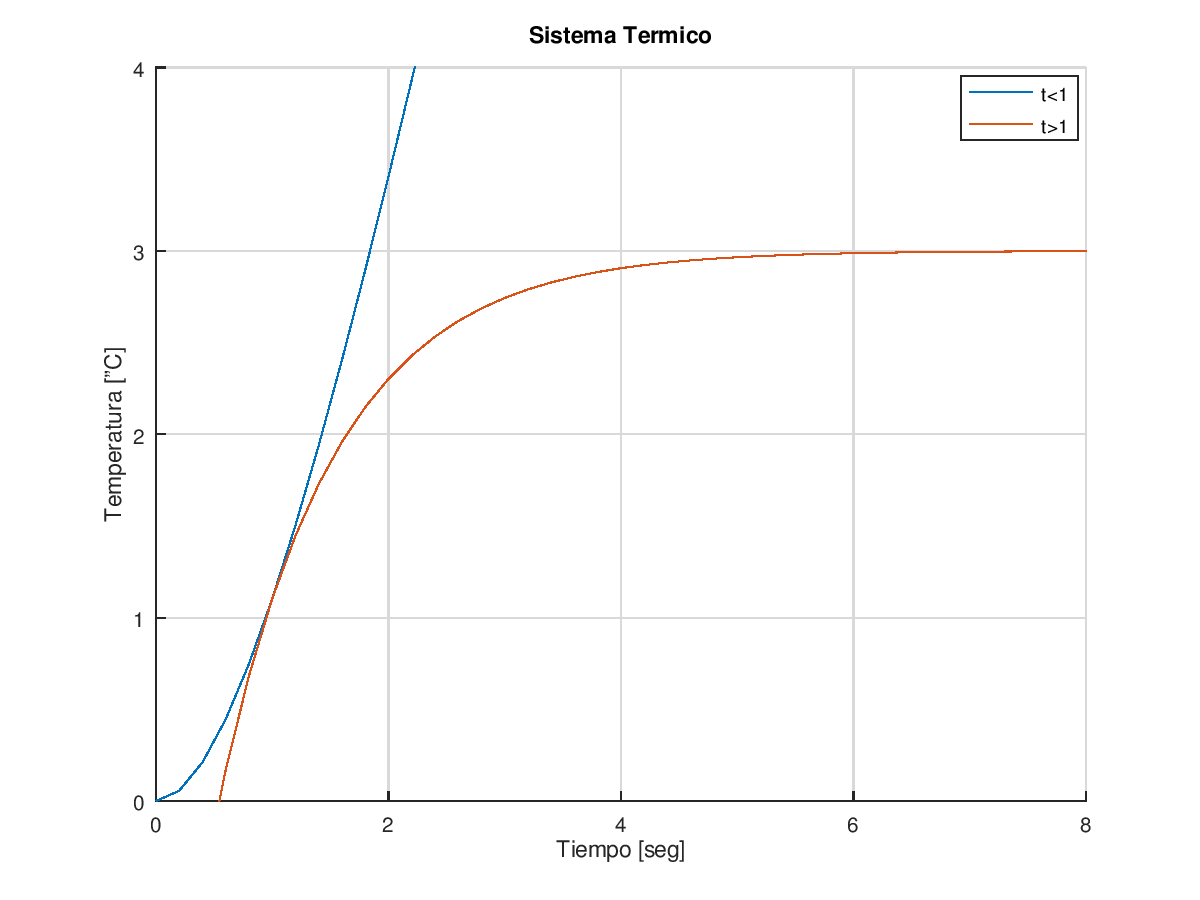
\includegraphics[width = 400pt]{imagenes/termotanqueTermico.png}
\caption{\small Comportamiento del sistema Termico.}
\label{red}
\end{center}
\end{figure}

%%%%%%%%%%%%%%%%%%%%%%%%%%%%%%%%%%%%%%%%%%%%


%\newpage
%\section{Soporte de la pierna del cuerpo humano}

%Para el análisis de este modelo se toman las sigueintes pautas:\par
%\begin{itemize}
%\item Se ignora la fuerza peso. Esto significa que se considera el sistema en equilibrio y al mismo se le aplica una fuerza externa.
%\item Aunque se corresponde con un sistema mecanico se realizara el estudio considerando su equivalencia electrica.
%\end{itemize}

%El sistema se corresponde con una fuerza externa aplicada sobre una $M_{1}$\p, que a su ves transfiere de forma amortiguada (ley de Hook) la misma a otra masa $M_{2}$. Esta ultima descarga la solicitacion amortiguando una parte (ley de Stokes) y disipando el resto de la misma.\p

%El circuito resultante sera:\p


\end{document}
